\documentclass[12pt,fleqn]{article}\usepackage{../../common}
\begin{document}
İlişkisel Madencilik (Association Mining)

İkisel Matris Ayrıştırması (Binary Matrix Factorization)

Veri madenciliği denince pek çok kişinin aklına gelen ilk örnek, aslında,
sık bulunan öğe kümeleri (frequent itemsets) örneğidir: "filanca ülkeden
sitemize gelen müşterilerin aynı zamanda vs özelliklerinin olduğunu da
keşfettik" gibi. 

Benzer bir örnek, ki bu alan öğe kümelerinin aslında en önemli çıkış
sebeplerinden birisidir, alışveriş sepeti analizidir. Müşterinin her
alışverişinde sepetinde belli mallar vardır, ve bu malların hangilerinin aynı
anda, aynı sepette olduğu analiz edilmeye uğraşılır. Eğer sürekli ekmek ve reçel
aynı anda alınıyorsa, bu bilgi kullanılarak belki malların daha iyi
konumlandırılması yapılacaktır, vs. Sık bulunan öğe kümeleri teknikleri bazen
değişik adlar altında da geçebiliyor, mesela ilişki madenciliği (association
mining) gibi. Algoritma olarak kullanılan pek çok teknik var, APriori iyi
bilinenlerden, FPGrowth ondan daha hızlı çalışan ve daha tercih edilen bir
teknik. İstatistiki bir teknik olan Çok Boyutlu Bernoulli Karışımları da bu
alanda kullanılan bir yaklaşım.

Bir diğer alternatif ikisel matris ayrıştırması (binary matrix
factorızation -BMF-) kullanmaktır [3]. Aynen SVD'de olduğu gibi BMF de bir
matrisi ayrıştırır, fakat üç matris yerine iki matrise ayrıştırır ve hem
sonuç matrisi hem de ayrıştırılan matrisler sadece 0 ya da 1 değerini
taşıyabilirler. Yani bu ayrıştırma sonuç matrislerinin ikisel olmasını
mecbur tutar, negatif olmayan matris ayrıştırmasının (non-negative matrix
factorızation) sonuç matrisinin pozitif değerler taşımasını mecbur kılması
gibi. Bunlar birer kısıtlama (constraint) ve bu sonuç o kısıtlamalara göre
ortaya çıkıyor. {\em Dikkat}: BMF için toplama işlemi $1+0 = 1, 1+1=1, 0+0
= 0$ olarak tekrar tanımlanır, yani mantıksal OR işlemi haline gelir.

Ayrıştırma öncesi hangi kerte (rank) $k$ değerine geçmek istediğimizi biz
belirtiriz. BMF'nin öğe kümeleri madenciliği için faydası şurada: öğe
kümeleri ararken baktığımız öğeler kategorik şeylerdir, alışveriş sepeti
örneğinde mesela ekmek, reçel gibi. Kategorik öğeleri daha önce 1-hot
kodlaması (encoding) ile 1/0 değerleri taşıyan yeni kolonlara
geçirebildiğimizi görmüştük. Yani tamamen kategorik değerler taşıyan
veriler tamamen 1/0 taşıyacak şekilde tekrar kodlanabilir, yani ikisel
matris haline getirilebilir. Bu ikisel matrisi ayrıştırdığımız zaman ve
kendileri de ikisel olan iki yeni matris elde ettiğimizde ise bir anlamda
boyut indirgemesi yapmış oluruz, yani sanki ana matrisi ``özetleriz''. İşte
bu özet, özellikle çarpılan ``baz'' matris, öğe kümelerinin hangileri
olduğu hakkında ipuçları içeriyor olabilir.

Bir örnek üzerinde görelim, mesela altta Alice (A), Bob Marley (B) ve Prens
Charles (C) verileri var. Bu kişiler için saçı uzun mu (long-haired), ünlü
mü (well-known) ve bay mı (male) verileri var. 

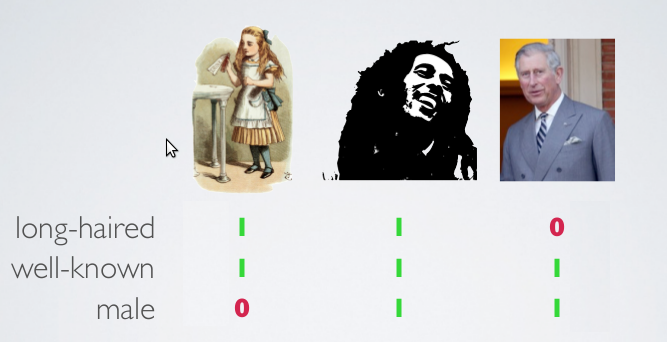
\includegraphics[height=5cm]{abc.png}

Bu matris üzerinde ikisel ayrıştırma yaparsak, $k=2$


\includegraphics[height=2cm]{abc_res.png}

Eğer kontrol etmek istersek, matris çarpımı yapmamız gerekir, bunun için

\begin{minted}[fontsize=\footnotesize]{python}
a = np.array([[1,  0],
               [1,  1],
               [0,  1]], dtype=bool)
b = np.array([[1,  1,  0],
               [0,  1,  1]], dtype=bool)

print np.dot(a,b)
\end{minted}

\begin{verbatim}
[[ True  True False]
 [ True  True  True]
 [False  True  True]]
\end{verbatim}

0 ve 1 değerleri görmek için 1 ile çarpmak yeterli

\begin{minted}[fontsize=\footnotesize]{python}
print 1*np.dot(a,b)
\end{minted}

\begin{verbatim}
[[1 1 0]
 [1 1 1]
 [0 1 1]]
\end{verbatim}

Sonuç başlangıç matrisi ile aynı, demek ki \verb!bool! tipi matris
tanımlayınca Numpy çarpımı \verb!dot!, çarpım sırasındaki toplama işlemi
için aritmetik toplama yerine VEYA (OR) kullanması gerektiğini anladı.

Şimdi ayrıştırmayı analiz edelim, özellikle sol taraftaki çarpılan ``baz''
matrise bakalım.. [6] yazısından hareketle, bu yazıdaki kolon kombinasyon
bakışını kullanalım (tabii toplamanın BMF için OR olduğunu unutmadan), o
zaman soldaki baz matrisin dikey, kolon bazlı olarak, bir özet olduğunu
görebiliyoruz. Çünkü çarpan sağ taraf bu kolonları alıp onları belli
şekillerde ``kombine ederek'' nihai (orijinal) matrisi ortaya
çıkartabilmeli. Bu sebeple soldaki çarpılan matris bir özet olmalı / baz
oluşturmalı, ve bunun yan etkisi olarak kolonlardaki değerlerde belli bir
kalıp / örüntü (pattern) olmalı. O zaman her baz kolonunda birbiriyle
alakalı olan ögeler aynı anda 1 değeri taşıyor olacaktır.

Sonuca göre uzun saçlı ve ünlü olmak (1. kolon) arasında bağlantı varmış ,
ayrıca erkek olmak ve ünlü olmak (2. kolon) arasında da bağlantı varmış :)
Veriye göre böyle en azından.. Bu sonucu orijinal matrise bakarak ta
kontrol edebiliriz.

Ayrıştırma Kodlaması 

BMF özel bir hesaptır ve Numpy / Scipy içinde mevcut değildir, ayrı bir
kütüphane kullanmak gereklidir, \verb!nimfa! paketi içinde gerekli kodlar
var. Kurduktan sonra üstteki örneği şöyle çözebiliriz;

\begin{minted}[fontsize=\footnotesize]{python}
import nimfa
import pandas as pd
import scipy.sparse as sp

def __fact_factor(X):
    return X.todense() if sp.isspmatrix(X) else X

A = np.array([[1., 1., 0],
              [1., 1., 1.],
              [0, 1., 1.]])

fctr = nimfa.mf(A,
              seed = "nndsvd", 
              rank = 2, 
              method = "bmf", 
              max_iter = 40, 
              initialize_only = True,
              lambda_w = 1.1,
              lambda_h = 1.1)

res = nimfa.mf_run(fctr)

threshold = 0.2
res1 = __fact_factor(res.basis())
res2 = __fact_factor(res.coef())
res1 = np.abs(np.round(res1 - 0.5 + threshold))
res2 = np.abs(np.round(res2 - 0.5 + threshold))
res1 = pd.DataFrame(res1, index=['long-haired','well-known','male'])
res2 = pd.DataFrame(res2, columns=['A','B','C'])
print res1
print '\n'
print res2
\end{minted}

\begin{verbatim}
             0  1
long-haired  1  0
well-known   1  1
male         0  1


   A  B  C
0  1  0  0
1  0  1  1
\end{verbatim}

Sonuç neredeyse tıpatıp aynı; sadece çarpan matriste [0,B] kordinatı 1
değil, fakat bize lazım olan baz matris aynı çıktı. 

BMF hakkında bazı ek bilgiler: [2]'ye göre en az hatalı BMF hesaplamak
NP-hard zorluğunda, yani 3SAT gibi, ya da Seyahat Eden Satış Elemanı
(Traveling Salesman) problemi gibi ki bu problemler kombinatoryel
(combinatorial) optimizasyon problemleridir; çözüm için tüm olasılıklar
denendiği ve kısayolun mevcut olmadığı çeşitten problemler. Fakat
yaklaşıksal BMF metotları oldukça hızlıdır, ayrıca seyreklik çok fark
yaratıyor (pozitif anlamda) ki kategorik veriler gerçek dünyada çoğunlukla
seyrek olarak görülüyor. Eldeki 2000 tane mal çeşidi içinden bir sepette
ancak 5-10 tane ürün oluyor mesela, tüm 2000 tane malı bir sepete koymak
mümkün değil.

FPGrowth


Öğe kümeleri bulmak için BMF haricinde bir yöntem FPGrowth yöntemidir
[1,2]. Bu yöntem önce her ögeden (tek başına) kaç tane olduğunu sayar,
belli bir eşik değeri \verb!minsup! altında olanları atar, sonucu
sıralar. Bu liste bir yapısına işaret eden bir başlık yapısı haline
gelir. Ağacın kendisini oluşturmak için veri satırları teker teker işlenir,
her satırdaki her öge için başlık yapısındaki en fazla değeri taşıyan öğe
önce olmak üzere tepeden başlanıp alta doğru uzayan bir ağaç yapısı
oluşturulur. Ağaçtaki her düğüm altındaki düğümün sayısal toplamını
taşır. Madencilik için alttan başlanarak yukarı doğru çıkılır (amaç en üste
ulaşmak) ve bu sırada öğeler \verb!minsup! altında ise, atılırlar. Sonuçta
ulaşılan ve atılmayan yollar bir öğe kümesini temsil ederler. 

Örnek verisi olarak alttakini kullanalım,

\begin{minted}[fontsize=\footnotesize]{python}
data = [
['outlook=sunny', 'temparature=hot', 'humidity=high', 'windy=false', 'play=no'],
['outlook=sunny', 'temparature=hot', 'humidity=high', 'windy=true', 'play=no'],
['outlook=overcast', 'temparature=hot', 'humidity=high', 'windy=false', 'play=yes'],
['outlook=rainy', 'temparature=mild', 'humidity=high', 'windy=false', 'play=yes'],
['outlook=rainy', 'temparature=cool', 'humidity=normal', 'windy=false', 'play=yes'],
['outlook=rainy', 'temparature=cool', 'humidity=normal', 'windy=true', 'play=no'],
['outlook=overcast', 'temparature=cool', 'humidity=normal', 'windy=true', 'play=yes'],
['outlook=sunny', 'temparature=mild', 'humidity=high', 'windy=false', 'play=no'],
['outlook=sunny', 'temparature=cool', 'humidity=normal', 'windy=false', 'play=yes'],
['outlook=rainy', 'temparature=mild', 'humidity=normal', 'windy=false', 'play=yes'],
['outlook=sunny', 'temparature=mild', 'humidity=normal', 'windy=true', 'play=yes'],
['outlook=overcast', 'temparature=mild', 'humidity=high', 'windy=true', 'play=yes'],
['outlook=overcast', 'temparature=hot', 'humidity=normal', 'windy=false', 'play=yes'],
['outlook=rainy', 'temparature=mild', 'humidity=high', 'windy=true', 'play=no']
]
\end{minted}

Hava ile alakalı bazı veriler [1] bunlar; bu veriler tahmin (outlook),
sıcaklık (temparature), nem (humidity), rüzgar (windy), dışarıda oyun
oynayan var mı (play). Mesela ilk satırda tahmin güneşli, ısı sıcak, nem
yüksek, rüzgar yok ve oyun oynayan yok. Bu şekilde bir sürü satır. Biz bu
veride bir kalıp olup olmadığına bakacağız. [2]'deki kodu [1]'den aldığımız
üstteki veriye uygularsak, sonuç şöyle:

\begin{minted}[fontsize=\footnotesize]{python}
import fp
items = fp.fpgrowth(data, minsup=6)
for x in items:
    if len(x) > 1: print x
\end{minted}

\begin{verbatim}
<fp.node instance at 0x5017ef0>
   Null Set   1
     play=yes   9
       humidity=high   1
         windy=true   1
           temparature=mild   1
       windy=false   6
         humidity=high   2
           temparature=mild   1
         humidity=normal   4
           temparature=mild   1
       humidity=normal   2
         windy=true   2
           temparature=mild   1
     humidity=high   2
       windy=true   2
         temparature=mild   1
     windy=false   2
       humidity=high   2
         temparature=mild   1
     humidity=normal   1
       windy=true   1
   Null Set   1
     play=yes   6
   Null Set   1
     play=yes   6
set(['play=yes', 'humidity=normal'])
set(['play=yes', 'windy=false'])
\end{verbatim}

Bulunan sonuçlar iki tane (tek öğeli sonuçlar da var ama onları
eledik). Bunlar hakikaten veri içindeki kalıpları temsil ediyorlar. Fena
değil. 

Kıyas için BMF üzerinden madencilik yapalım. Önce 1-hot kodlaması yapalım,
ve örnek için bir veri satırını ekrana basalım,

\begin{minted}[fontsize=\footnotesize]{python}
from sklearn.feature_extraction import DictVectorizer
import pandas as pd, re

def one_hot_dataframe(data, cols, replace=False):
    vec = DictVectorizer()
    mkdict = lambda row: dict((col, row[col]) for col in cols)
    tmp = data[cols].apply(mkdict, axis=1)
    vecData = pd.DataFrame(vec.fit_transform(tmp).toarray())
    vecData.columns = vec.get_feature_names()
    vecData.index = data.index
    if replace is True:
        data = data.drop(cols, axis=1)
        data = data.join(vecData)
    return (data, vecData, vec)

cols = ['outlook','temparature','humidity','windy','play']
df = pd.DataFrame(data,columns=cols)
# kolon ismini veriden cikart, cunku tekrar geri koyulacak
# fpgrowth icin veri icinde olmasi lazim
df = df.applymap(lambda x: re.sub('.*?=','',x))
df2, _, _ = one_hot_dataframe(df, cols, replace=True)
# tek ornek ekrana bas
print df2.ix[0]
\end{minted}

\begin{verbatim}
humidity=high       1
humidity=normal     0
outlook=overcast    0
outlook=rainy       0
outlook=sunny       1
play=no             1
play=yes            0
temparature=cool    0
temparature=hot     1
temparature=mild    0
windy=false         1
windy=true          0
Name: 0, dtype: float64
\end{verbatim}

Şimdi BMF işletelim, $k=4$

\begin{minted}[fontsize=\footnotesize]{python}
import nimfa
import scipy.sparse as sp

def __fact_factor(X):
    return X.todense() if sp.isspmatrix(X) else X

fctr = nimfa.mf(np.array(df2).T, seed = "nndsvd", 
              rank = 4, method = "bmf", 
              max_iter = 40, initialize_only = True,
              lambda_w = 1.1, lambda_h = 1.1)

res = nimfa.mf_run(fctr)

threshold = 0.2
res1 = __fact_factor(res.basis())
res2 = __fact_factor(res.coef())
res1 = np.abs(np.round(res1 - 0.5 + threshold))
res2=  np.abs(np.round(res2 - 0.5 + threshold))
res1 = pd.DataFrame(res1,index=df2.columns)
print res1
\end{minted}

\begin{verbatim}
                  0  1  2  3
humidity=high     1  0  0  1
humidity=normal   0  1  0  0
outlook=overcast  0  0  1  0
outlook=rainy     1  0  0  0
outlook=sunny     0  0  0  1
play=no           0  0  0  1
play=yes          0  1  1  0
temparature=cool  0  0  0  0
temparature=hot   0  0  0  0
temparature=mild  1  0  0  0
windy=false       0  0  1  0
windy=true        1  0  0  0
\end{verbatim}

Bu sonuçları kategoriksel hale çevirip tekrar ekrana basalım,

\begin{minted}[fontsize=\footnotesize]{python}
for i in range(4):
    print np.array(df2.columns)[res1.ix[:,i] == 1]
\end{minted}

\begin{verbatim}
['humidity=high' 'outlook=rainy' 'temparature=mild' 'windy=true']
['humidity=normal' 'play=yes']
['outlook=overcast' 'play=yes' 'windy=false']
['humidity=high' 'outlook=sunny' 'play=no']
\end{verbatim}

1. sonuç atlanabilir, buradaki ``kalabalık'' orada bir kalıp olmadığına
dair bir işaret. Ayrıştırma sonucu bu tür kolonlar ortaya çıkabilir, diğer
kolonlardaki kalıplar bütünü temsil etmeye {\em tam} yetmemişse, arta kalan
her türlü gereklilik bir yerlere tıkılabiliyor, bu normal. 2. sonuç
FPGrowth sonucunda var, güzel. 3. sonuç ta neredeyse aynı, sadece ek olarak
\verb!outlook=overcast! var. Fakat, 3. sonuç aslında önemli bir kalıp
içeriyor olabilir, yani kalması daha iyi olur.

4. sonuç ise çok önemli bir kalıp ve FPGrowth bunu tamamen kaçırmış!

Sebep FPGrowth'un çözüme lokal olarak erişmeye çalışıyor olması, kıyasla
BMF bütüne (global) bakıyor [3]. Bu ne demektir? Bir ayrıştırmanın ne
olduğunu düşünürsek, bir matrisi oluşturan çarpımı ayrıştırıyoruz ve bu
ayrıştırma olduktan sonra iki matris elde ediyoruz. Bu iki matris özgündür 
(unique). Yani belli bir ikisel matrisi oluşturan çarpım sadece tek bir
şekilde olabilir. Buradan hareketle diyebiliriz ki bu ayrıştırma bütünü
göze alarak yapılmalıdır, sağı, solu tutan ama köşesi tutmayan bir
ayrıştırma olmaz. Bu sebeptendir ki ayrıştırma çözümünden belli bir
kapsayıcılık bekleyebiliriz.

FPGrowth ise olaya yerel bakıyor; ağaç oluştururken değişik bir sıra takip
edilirse mesela değişik ağaçlar ortaya çıkabilir. Ayrıca her önemli ilişki
muhakkak özgün bir dal yapısında olmayabilir. Madencilik algoritması alt
dallardan başlar ve yukarıya doğru çıkar, fakat bu her zaman iyi bir yöntem
midir?

Kodlama Notları

Şu kod \verb!np.round(num - 0.5 + threshold)! kullanımı yuvarlama
(rounding) yapıyor, çünkü Nimfa 1 değeri yerine 0.9, 0.8 gibi değerler
üretebiliyor, ayrıca 0.1 gibi değerler de oluyor. Biz bildiğimiz yuvarlama
\verb!.5!  sonrası üzerini 1 yapmak yerine belli bir eşik değeri
(threshold) üzerinden yuvarlama yaptık. Yani eşik=0.2 ise 0.7 alta
yuvarlanır ve 0 olur, 0.9 eşik üstünde olduğu için üste yuvarlanır 1 olur.

BMF için kerte $k$ kullanıcı tarafından seçilmeli, ama bu durum SVD, ya da
GMM ile kümeleme gibi diğer yapay öğrenim metotlarından farklı değildir. Bu
oynanması gereken, keşfedilmesi gereken bir değer.

Çok Değişkenli Bernoulli Karışımı Kümelemesi ile İlişkisel Madencilik

Bir diger yaklasim kümeleme üzerinden kural çıkartmak. Örnek veri olarak
[7] yazısındanki Movielens 1M verisini kullanacağız. Ayrıca bu verideki
posta kodu (zip) ve meslek (occupation) verisine README'ye ve bir Internet
sitesine [4] danışarak sözel açıklamalarını koyduk. Böylece sonuçları
yorumlamak çok daha kolay olacak.

İlişkilerin keşfi için çok değişkenli Bernoulli modelini kullanacağız, ki
[8] yazısında bu kümeleme yöntemi işlendi. CDBK kullanmak için veriyi 0/1
bazına indirgeyeceğiz (ki verinin büyük bir kısmı zaten bu durumda)
ardından CDBK'yı veriye uyduracağız, ve karışım öğeleri $\theta_k$'lerin
bir nevi ``şablon'' oluşturması sebebiyle ilişki keşfini bu şablonlar
üzerinden yapmaya uğraşacağız.

\begin{minted}[fontsize=\footnotesize]{python}
import pandas as pd, zipfile
import sys; sys.path.append('../stat_mixbern')
import mixbern

unames = ['user_id', 'gender', 'age', 'occupation', 'zip']
rnames = ['user_id', 'movie_id', 'rating', 'timestamp']
mnames = ['movie_id', 'title', 'genres']
with zipfile.ZipFile('../stat_ratings/ml1m.zip', 'r') as z:
    users = pd.read_table(z.open('users.dat'), sep='::', header=None,names=unames)
    ratings = pd.read_table(z.open('ratings.dat'), sep='::', header=None,names=rnames)
    movies = pd.read_table(z.open('movies.dat'), sep='::', header=None,names=mnames)
\end{minted}

\begin{minted}[fontsize=\footnotesize]{python}
occup_map = \
{ 0:  "other" or not specified,1:  "academic/educator",
  2:  "artist",3:  "clerical/admin",
  4:  "college/grad student",5:  "customer service",
  6:  "doctor/health care",7:  "executive/managerial",
  8:  "farmer",9:  "homemaker",
  10:  "K-12 student", 11:  "lawyer",
  12:  "programmer",13:  "retired",
  14:  "sales/marketing",15:  "scientist",
  16:  "self-employed",17:  "technician/engineer",
  18:  "tradesman/craftsman",19:  "unemployed",
  20:  "writer"}

zip_map = \
{ 0: 'Northeast', 1: 'NY Area', 2: 'DC', 3: 'Florida', 4: 'Michigan/Ohio', 
  5: 'North', 6: 'Illinois', 7: 'Texas / Arkansas', 8: 'Nevada / Utah', 
  9: 'California / Alaska'}

from sklearn.feature_extraction import DictVectorizer
def one_hot_dataframe(data, cols):
    vec = DictVectorizer()
    mkdict = lambda row: dict((col, row[col]) for col in cols)
    tmp = vec.fit_transform(data[cols].to_dict(outtype='records')).toarray()
    vecData = pd.DataFrame(tmp)
    vecData.columns = vec.get_feature_names()
    vecData.index = data.index
    data = data.drop(cols, axis=1)
    data = data.join(vecData)
    return data

df = users.copy()
df['occupation'] = df.apply(lambda x: occup_map[x['occupation']], axis=1)
df['zip2'] = users['zip'].map(lambda x: int(str(x)[0]))
df['zip2'] = df.apply(lambda x: zip_map[x['zip2']], axis=1)
df['age2'] = pd.qcut(df['age'],5)
df = one_hot_dataframe(df,['occupation','gender','zip2','age2'])
df = df.drop(['zip','age'],axis=1)
df = df.set_index('user_id')
\end{minted}

ZIP kodları altta gösteriliyor

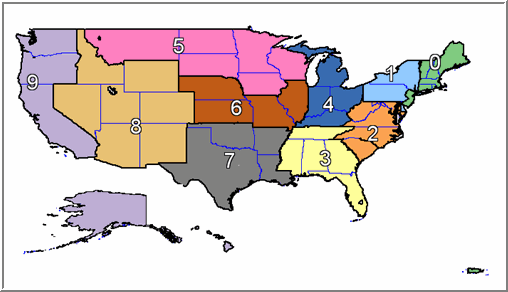
\includegraphics[height=7cm]{zip_code_zones.png}

Şimdi hangi film genre'sinin (türünün) kullanıcı tarafından kaç kez alınmış
olduğunu özetleyip kullanıcı verisine bitişik olarak ekleyeceğiz. 

\begin{minted}[fontsize=\footnotesize]{python}
genre_iter = (set(x.split('|')) for x in movies.genres)
genres = sorted(set.union(*genre_iter))
dummies = pd.DataFrame(np.zeros((len(movies), len(genres))), columns=genres)
for i, gen in enumerate(movies.genres):
   dummies.ix[i, gen.split('|')] = 1
movies_windic = movies.join(dummies.add_prefix('Genre_'))
movies_windic = movies_windic.drop(['title','genres'],axis=1)
joined = ratings.merge(movies_windic, left_on='movie_id',right_on='movie_id')
genres = joined.groupby('user_id').sum()
genres = genres.drop(['movie_id','rating','timestamp'],axis=1)
X = pd.merge(df, genres, left_index=True, right_index=True,how='left')
print X.shape
\end{minted}

\begin{verbatim}
(6040, 56)
\end{verbatim}

En iyi küme sayısı nedir? Bunun için mümkün tüm küme sayılarını deneriz,
AIC sonuçlarına bakarız, sonuçlar arasından düşüş ardından ilk çıkış olduğu
anı en iyi küme sayısı olarak kullanırız. 

\begin{minted}[fontsize=\footnotesize]{python}
iter=40; eps=1e-15; attempts=5
for K in range(5,16):
    lR,lPi,lP,lbest,aic = mixbern.EMmixtureBernoulli(X,K,iter,eps,attempts)
    print K,aic
\end{minted}

\begin{verbatim}
5,173126.633281
6,172007.606772
7,170285.383519
8,169043.301004
9,168457.12051
10,167463.532805
11,167253.486012
12,166290.598818
13,165764.506989
14,164964.964083
15,164989.85056
16,164321.25051
\end{verbatim}

Sonuçlara göre $K=14$ bu çıkış anını yakalar. Bu sayıyla tekrar kümelemeyi
işletelim,

\begin{minted}[fontsize=\footnotesize]{python}
iter=40; eps=1e-15; attempts=5; K=14
lR,lPi,lP,lbest,aic = mixbern.EMmixtureBernoulli(X,K,iter,eps,attempts)
rules = np.exp(lP)
\end{minted}

\begin{minted}[fontsize=\footnotesize]{python}
def print_rule(j):
    for i,r in enumerate(rules[j]): 
         if r > 0.5: print X.columns[i], r
\end{minted}

Şimdi bazı kuralları ekrana basalım,

\begin{minted}[fontsize=\footnotesize]{python}
print_rule(0)
\end{minted}

\begin{verbatim}
age2=(25, 35] 1.0
gender=M 1.0
Genre_Action 0.997646429789
Genre_Adventure 0.976908591072
Genre_Animation 0.73312197406
Genre_Children's 0.815806962254
Genre_Comedy 1.0
Genre_Crime 0.888200034236
Genre_Drama 1.0
Genre_Fantasy 0.759168898223
Genre_Film-Noir 0.535819148049
Genre_Horror 0.859145011653
Genre_Musical 0.704293299334
Genre_Mystery 0.735085517947
Genre_Romance 0.999999999621
Genre_Sci-Fi 0.98865549819
Genre_Thriller 1.0
Genre_War 0.948000910806
Genre_Western 0.590038323721
\end{verbatim}

25 ila 35 yaş arasındaki erkekler komedi ve aksiyon çok seviyorlar, en çok
beğendiklerinin arasında en alt sırada Western var. İlginç.

\begin{minted}[fontsize=\footnotesize]{python}
print_rule(1)
\end{minted}

\begin{verbatim}
age2=(18, 25] 1.0
gender=M 1.0
Genre_Action 0.999999916342
Genre_Adventure 0.968035357641
Genre_Animation 0.618607301467
Genre_Children's 0.733114850427
Genre_Comedy 1.0
Genre_Crime 0.895303009556
Genre_Drama 1.0
Genre_Fantasy 0.621607330213
Genre_Horror 0.826409070694
Genre_Mystery 0.667105230382
Genre_Romance 0.962487486107
Genre_Sci-Fi 0.981703990034
Genre_Thriller 0.999998477836
Genre_War 0.884260074733
\end{verbatim}

Daha dar bir yaş aralığı 18-25 yaş grubu, komedi, dram, aksiyon, gerilim
var, en az sevilen filmler bu sefer animasyon.

\begin{minted}[fontsize=\footnotesize]{python}
print_rule(2)
\end{minted}

\begin{verbatim}
gender=F 1.0
Genre_Action 1.0
Genre_Adventure 0.997753376918
Genre_Animation 0.925605697933
Genre_Children's 0.989223061984
Genre_Comedy 0.999411653044
Genre_Crime 0.978893423529
Genre_Drama 1.0
Genre_Fantasy 0.890898944372
Genre_Film-Noir 0.810452619282
Genre_Horror 0.901607018088
Genre_Musical 0.93690169152
Genre_Mystery 0.949990841295
Genre_Romance 1.0
Genre_Sci-Fi 0.999467975234
Genre_Thriller 0.997148167548
Genre_War 0.987837234705
Genre_Western 0.801075654907
\end{verbatim}

Bayanlar için (yaş grubu yok dikkat), üstte aksiyon var, ama romantik
filmler de en üstte. 

Şu da ilginç bir bulgu; meslek kolları ve adres verilerini analize dahil
etmiş olmamıza rağmen kümelerin şablonu içinde hiçbiri yok! Demek ki
meslekler, adresler film beğenisinde fark yaratmıyor.

Üstteki analiz müşteri bilgisine müşteri seviyesinde baktı. Eğer işlemsel
(transactional) bir analiz yapıyor olsaydık, yaklaşım benzer olacaktı,
sadece veri odağı biraz farklı olurdu; müşterilerin her alışveriş
sepetlerine bakılacaktı mesela, bir sepete koyulan mesela ekmek, çikolata,
su, bir diğerine koyulan ekmek, su, biberon gibi alımlar bir satırda 1 ile
işaretli, diğerleri 0 ile işaretli olacaktı, ve kümeleme algoritması bu çok
boyutlu Bernoulli veriye bir uyum yapıp şablonları raporlayacaktı.

İlginçlik - İstatistiki Ölçüt

Kümeleri uydurduktan sonra bile bu kümelerin içinde hangisinin ``daha iyi''
olduğunu bulmak için istatistiki ölçüt kullanmak faydalı olabilir. Hatta
birazdan bahsedeceğimiz teknik aslında her türlü ilişki madenciliği
yaklaşımı için faydalı, çünkü hangi teknik olursa olsun bize verinin belli
bir grubunu ``önemli'' olarak gösterecek. Ardından biz bu grubu alıp onun
ne kadar önemli olduğunun ölçütünü hesaplayabileceğiz.

Teknik şöyle: İstatistiki testlerden [9] yazı bölümünü hatırlarsak, bir
ideal dağılım vardı, ve eldeki verinin bu ideale olan yakınlığını
ölçüyorduk. Chi Kare testi ayrıksal bazda işliyordu, eğer eldeki sürekli
fonksiyon bazlı bir dağılım ise onun ideal hesaplarını kutucuklara
bölüştürüyorduk.

İlişkisel madencilikte elde ettiğimiz kural bir vektör içinde 0/1 değerleri
olacak. Yaklaşım şöyle; önce verideki her kolonun tek başına oranını
buluruz. Bu oranlar her kolon ``dağılımının'' birbirinden bağımsız farz
edildiği ``idealize'' ortamın ölçütleri olacaklar. Veri mesela şöyle,

\begin{minted}[fontsize=\footnotesize]{python}
data = [[1,1,0,0,1],
        [1,0,0,0,0],
        [1,0,0,1,1],
        [1,1,0,1,1],
        [1,1,1,0,1],
        [0,0,1,1,0],
        [0,1,1,0,0]
        ]
data = np.array(data)
sums = data.sum(axis=0)
means = data.mean(axis=0)
print 'toplam', sums
print 'ortalama', means
\end{minted}

\begin{verbatim}
toplam [5 4 3 3 4]
ortalama [ 0.71428571  0.57142857  0.42857143  0.42857143  0.57142857]
\end{verbatim}

Şimdi bulunan kurallardan birini, diyelim \verb![1,1,0,0,1]!, ana veride en
fazla 1 sayısına tekabül eden kolonunu seçeriz, ve bu kolonun 1 olduğu tüm
satırları bir alt küme olarak toparlarız. Bu alt kümede diyelim 5 tane
satır var, ve kuralın diğer ögeleri 1. haricinde 2. ve 5.  kolonun da '1'
değerinde olması. O zaman, toplam 5 satır için 2. ve sonuncu satırda 5*0.57
ve 5*0.57 tane satır olmalı. Sıfır hipotezi bağımsızlık olduğu için bu
``beklenen (expected)'' sayı. Diğer yandan gerçek rakamlar var, bu rakamlar
alt kümedeki '1' değerlerinin toplamı, ki bu da ``görünen (observed)''
sayı. Bu iki vektör üzerinden chi kare değerini hesaplıyoruz [5, sf. 391],

$$ \chi^2 = \sum_i \frac{(O_i-E_i)^2}{E_i} $$

$\chi^2$'nin serbestlik derecesi 3-1=2 (çünkü kuralda 3 tane kolon var,
1. kolonu alt kümeyi bulmak için kullandık). p-değeri ne kadar yüksek ise
kural o kadar ilginç diyebiliriz.

\begin{minted}[fontsize=\footnotesize]{python}
from scipy.stats.distributions import chi2

def interesting(rule): 
     idx = (sums*rule).argmax()
     subset = data[data[:,idx] == 1]
     print subset
     print subset[:,rule==1]
     obs = subset[:,rule==1].sum(axis=0)
     exp = len(subset)*means[rule==1]
     print 'gorunen (observed)', obs
     print 'beklenen (expected)', exp
     chi = np.sum((obs-exp)**2 / exp)
     dof = rule.sum()-1
     print 1-chi2.cdf(chi,dof)

rule = np.array([1,1,0,0,1])
interesting(rule)
\end{minted}

\begin{verbatim}
[[1 1 0 0 1]
 [1 0 0 0 0]
 [1 0 0 1 1]
 [1 1 0 1 1]
 [1 1 1 0 1]]
[[1 1 1]
 [1 0 0]
 [1 0 1]
 [1 1 1]
 [1 1 1]]
gorunen (observed) [5 3 4]
beklenen (expected) [ 3.57142857  2.85714286  2.85714286]
0.595795886519
\end{verbatim}

Bir başka kural deneyelim, 

\begin{minted}[fontsize=\footnotesize]{python}
rule = np.array([1,0,0,0,1])
interesting(rule)
\end{minted}

\begin{verbatim}
[[1 1 0 0 1]
 [1 0 0 0 0]
 [1 0 0 1 1]
 [1 1 0 1 1]
 [1 1 1 0 1]]
[[1 1]
 [1 0]
 [1 1]
 [1 1]
 [1 1]]
gorunen (observed) [5 4]
beklenen (expected) [ 3.57142857  2.85714286]
0.310494434317
\end{verbatim}

Bu daha az ilginçmiş. Hakikaten de ilk kuralın veriye bakarak daha ilginç
olduğunu söyleyebiliriz. 

Gösterdiğimiz tekniği film sonuçlarında kullanmadık, bunu ödev olarak
okuyucuya bırakıyoruz.

Kaynaklar

[1] Ian H. Witten, Eibe Frank, Mark A. Hall, {\em Data Mining Practical Machine Learning Tools and Techniques}

[2] Harrington, P., {\em Machine Learning in Action}

[3] Miettinen, {\em Boolean Matrix Factorizations}, \url{http://www.mpi-inf.mpg.de/~pmiettin/slides/BooleanMatrixFactorizationsForDataMining_Antwerp_slides.pdf}

[4] Zip boundary, {\em ZIP Code FAQs}, \url{http://www.zipboundary.com/zipcode_faqs.html}

[5] Rao, {\em Linear Statistical Inference and Its Applications}

[6] Bayramlı, Lineer Cebir, {\em Matris Çarpımı, Ders 1}

[7] Bayramlı, Istatistik, {\em Pivotlama}

[8] Bayramlı, Istatistik, {\em Çok Değişkenli Bernoulli Karışımı}

[9] Bayramlı, Istatistik, {\em Pearson Chi Kare Uyum Derecesi Testi}



\end{document}
